\documentclass[11pt]{article}
\usepackage[utf8]{inputenc}
\usepackage{listings}
\usepackage{xcolor}
\usepackage{graphicx}
\usepackage{amsmath}
\usepackage{algorithm}
\usepackage{algpseudocode}
\usepackage{graphicx}
\usepackage[a4paper, margin=1in]{geometry}
\usepackage{float}
\usepackage{comment}

% Custom style for function specifications
\lstdefinestyle{specification}{
    basicstyle=\ttfamily\bfseries\small, % Bold monospace for specs
    backgroundcolor=\color{gray!10},     % Light gray background
    frame=single,                        % Border around the spec
    keywordstyle=\color{blue}\bfseries,  % Keywords in bold blue
    commentstyle=\color{green!50!black}, % Comments in green
    numbers=none,                        % No line numbers
    showstringspaces=false
}

\title{Mechanical System}
\author{Daniel Yu}
\date{\today}

% Define code formatting

\begin{document}
\lstdefinestyle{ArduinoCode}{
    language=C++,
    basicstyle=\ttfamily\small,
    keywordstyle=\color{blue},
    commentstyle=\color{gray},
    stringstyle=\color{red},
    breaklines=true,
    numbers=left,
    numberstyle=\tiny\color{gray},
    frame=single,
}

\maketitle

\section{Introduction}
The goal is to have a mechanical system that do one SAR scan with related SAR parameters: $\Delta x, \Delta y, Points_{x}, Points_{y}$. 
\\\\
The mechanical system has a specified X and Y dimensions.\\
Two stepper motors are used for x-axis and y-axis. A stepper motor has two parameters, DIR and PUL(technically PUL$+$, but PUL$-$ is grounded). Relative to the mechanical system implementation of the previous group, these pins are connected to Arduino pins, and pushing high or low to them move the radar in a certain way. Specifically:\\
\begin{tabular}{|c|c|c|}
\hline
Motor Pins & HIGH & LOW \\ 
\hline
DIRx & Right & Left  \\ 
\hline
DIRy & Down & Up \\ 
\hline
PULx & Move 1 microstep & Not move \\ 
\hline
PULy & Move 1 microstep & Not move \\ 
\hline
\end{tabular}
\\\\
One stepper motor microstep corresponds to 0.04mm by the implementation of the mechancal sytem from the previous group.\\
Thus, the final program output will look something like this: \\
Set fixed values for parameters $\Delta x, \Delta y, Points_{x}, Points_{y}$:\\
Motor move with radar from origin to end(arbitarily specified, but should occupy the whole grid), completing one SAR scan. After completion, it returns to origin.\\
Additionally, it do so discretely with synchronization. Specifically:\\
Given $Points_{x}=N, Points_{y}=M, \Delta x=dim{X}/Points_{x}, \Delta y=dim{Y}/Points_{y}$\\
The mechanical system has a fixed dimension: around 40 cm x 40 cm\\
$\Delta x=P_{xi+1} - P_{xi}, i=1,2,...,N$\\\\

\algblock{Loop}{EndLoop}
\algrenewtext{Loop}[1]{\textbf{loop}} % Replaces 'While' with 'loop'
\algrenewtext{EndLoop}{\textbf{end loop}}
\begin{algorithm}
\caption{Implement this for now}
\begin{algorithmic}[1]
\Loop{traverse y}
    \Loop{traverse x}
        \State Traverse $P_{xi}$ to $P_{xi+1}$
        \State Stop motor, pause 2 sec
        \State Send prompt to console
    \EndLoop{ if reaches end of row}
    \State Move $\Delta y$
    \State Stop motor, pause 2 sec
    \State Send prompt to console
\EndLoop{ if reaches end of column}
\end{algorithmic}
\end{algorithm}

\begin{figure}[H] % Use 'H' to force placement exactly here
    \centering
    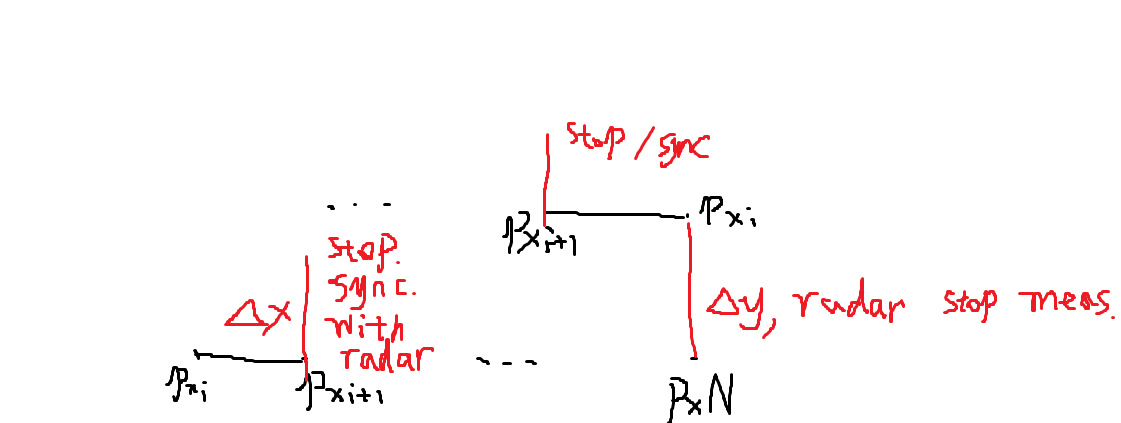
\includegraphics[width=0.6\textwidth, scale=3]{SARScanHow.png}
    \caption{Very Very Pretty Drawing On How This Works}
    \label{fig:art}
\end{figure}

\section{Implementation}
Check files, there are already things implemented
\begin{comment}
\begin{figure}[H]
\begin{lstlisting}[style=specification]
Function: step_x()

Description:
    move one motor microstep in the given direction in x(already done).
    motor moves on rising edge, do Pulse width modulation as fast as possible,
    reference provided spec sheet/tests

Preconditions:
    direction for x is initialized

Postconditions:
    motor movement in x
\end{lstlisting}
\end{figure}
\end{comment}

\section{Organization}
\begin{itemize}
    \item chill and have fun
    \item get all As for your summer classes
    \item finish this
\end{itemize}

\section{Deadline}
just do stuff bro.

\end{document}
